%convert -coalesce launch.gif launch_%d.png
\documentclass{beamer}

\newcommand{\VEV}[1]{\langle#1\rangle}
\newcommand{\sst}{\left(1-\frac{2M}{r}\right)}
\newcommand{\sh}{\mathrm{shell}}
\newcommand{\be}{\begin{equation}}
\newcommand{\ee}{\end{equation}}
\newcommand{\bue}{\begin{equation}}
\newcommand{\eue}{\end{equation}}
\newcommand{\bc}{\begin{center}}
\newcommand{\ec}{\end{center}}
\newcommand{\bea}[1]{\begin{eqnarray}\label{#1}}
\newcommand{\eea}{\end{eqnarray}}
\newcommand{\bua}{\begin{eqnarray*}}
\newcommand{\eua}{\end{eqnarray*}}
\newcommand{\dd}[2]{{{d#1}\over{d#2}}}
\newcommand{\ddt}[1]{\dd{#1}{t}}
\newcommand{\dddt}[1]{\dd{^2#1}{t^2}}
\newcommand{\aver}[1]{\langle{#1}\rangle}
\newcommand{\atom}[3]{\ifmmode^{#1}_{#2}{\rm{#3}}\else{$^{#1}_{#2}${#3}}\fi}
\newcommand{\electron}{\atom{~0}{-1}{e}}
\newcommand{\positron}{\atom{0}{0}{\bar{e}}}
\newcommand{\neutrino}{\atom{0}{0}{\nu_e}}
\newcommand{\photon}{\atom{0}{0}{\gamma}}
\newcommand{\antineutrino}{\atom{0}{0}{\bar{\nu}}}
\newcommand{\neutron}{\atom{1}{0}{n}}
\newcommand{\proton}{\atom{1}{1}{p}}
\newcommand{\hydrogen}{\atom{1}{1}{H}}
\newcommand{\deuterium}{\atom{2}{1}{H}}
\newcommand{\tritium}{\atom{3}{1}{H}}
\newcommand{\helium}{\atom{4}{2}{He}}
\newcommand{\hethree}{\atom{3}{2}{He}}

\renewcommand{\ss}{Schwarz\-schild }

\def\densu{kg/m$^3$} 
\def\rsol{R$_{\odot}$} 
\def\msol{M$_{\odot}$} 


\usetheme{Boadilla}
%\usepackage{multimedia}
%\usepackage{animate}
\usepackage{hyperref}
\usepackage{tikz}
\usepackage{cancel}
\usepackage{tikzsymbols}
\usepackage{ifthen}

%%%%mathcircled
\makeatletter
\newcommand\mathcircled[1]{%`
  \mathpalette\@mathcircled{#1}%
}
\newcommand\@mathcircled[2]{%
  \tikz[baseline=(math.base)] \node[draw,circle,red, thick, inner sep=2pt] (math) {$\m@th#1#2$};%
}
\makeatother
%%%%

%gets rid of bottom navigation bars
\setbeamertemplate{footline}[frame number]{}

%gets rid of bottom navigation symbols
\setbeamertemplate{navigation symbols}{}

%gets rid of footer
%will override 'frame number' instruction above
%comment out to revert to previous/default definitions
\setbeamertemplate{footline}{}

\definecolor{darkscarlet}{rgb}{0.34, 0.01, 0.1}
\definecolor{gold(metallic)}{rgb}{0.83, 0.69, 0.22}
\definecolor{green(ryb)}{rgb}{0.4, 0.69, 0.2}
\definecolor{darkorange}{rgb}{1.0, 0.55, 0.0}
\definecolor{amber}{rgb}{1.0, 0.75, 0.0}
\definecolor{bronze}{rgb}{0.8, 0.5, 0.2}
\definecolor{cadet}{rgb}{0.33, 0.41, 0.47}
\definecolor{silver}{rgb}{0.75, 0.75, 0.75}
\definecolor{turquoise}{rgb}{0.19, 0.84, 0.78}
\definecolor{uclagold}{rgb}{1.0, 0.7, 0.0}
\definecolor{urobilin}{rgb}{0.88, 0.68, 0.13}
\definecolor{vegasgold}{rgb}{0.77, 0.7, 0.35}
\definecolor{vanilla}{rgb}{0.95, 0.9, 0.67}
\definecolor{straw}{rgb}{0.89, 0.85, 0.44}
\definecolor{sunset}{rgb}{0.98, 0.84, 0.65}
\definecolor{brown(traditional)}{rgb}{0.59, 0.29, 0.0}
\definecolor{apricot}{rgb}{0.98, 0.81, 0.69}
\definecolor{darkblue}{rgb}{0,0,0.54}

\hypersetup{
    colorlinks=true,
    linkcolor=yellow,
    filecolor=magenta,      
    urlcolor=blue,
}

\let\hrefori\href
\renewcommand{\href}[2]{{\setlength{\fboxsep}{1pt}\colorbox{sunset}{\hrefori{#1}{#2}}}}


%title
\setbeamercolor{block title alerted}{fg=white,bg=cyan}
%body
\setbeamercolor{block body alerted}{fg=black!90,bg=yellow!60}

%title
\setbeamercolor{block title}{fg=black,bg=turquoise}
%body
\setbeamercolor{block body}{fg=yellow,bg=bronze}




\newcommand{\pagebutton}[1]{\setbeamertemplate{button}{\tikz\node[inner xsep = 5pt, draw = structure!90, fill = green(ryb), rounded corners = 8pt]{\color{amber}\Large\insertbuttontext};}\beamerbutton{#1}}

\newcommand{\choicebutton}[1]{\setbeamertemplate{button}{\tikz\node[inner xsep = 8pt, draw = structure!90, fill = vegasgold, rounded corners = 5pt]{\color{vanilla}\Large\insertbuttontext};}\beamerbutton{#1}}

\newcommand{\pagenobutton}[1]{\setbeamertemplate{button}{\tikz\node[inner xsep = 8pt, draw = structure!90, fill = apricot, rounded corners = 5pt]{\color{brown(traditional)}\Large\insertbuttontext};}\beamerbutton{#1}}

\newcommand{\headlinebutton}[1]{\setbeamertemplate{button}{\tikz\node[inner xsep = 8pt, draw = structure!90, fill = blue, rounded corners = 5pt]{\color{yellow}\Large\insertbuttontext};}\beamerbutton{#1}}

\newcommand{\forumbutton}{\href{https://astro-discourse.utenforuio.no/c/ast2000/sporsmal-til-forelesningsnotater-del-1a-1g/16}{\setbeamertemplate{button}{\tikz\node[inner xsep = 8pt, draw = structure!90, fill = darkblue, rounded corners = 5pt]{\color{yellow}\Large\insertbuttontext};}\beamerbutton{\textcolor{red}{\small FORUM}}}}

\newcommand{\curpage}{\pagenobutton{\small side \thepageno\  av \thenopages}}
\newcommand{\nextpage}{\refstepcounter{pageno}\pagenobutton{\small side \thepageno\  av \thenopages}}
\newcommand{\dnextpage}{\refstepcounter{pageno}\refstepcounter{pageno}\pagenobutton{\small side \thepageno\  av \thenopages}}

\newcommand{\lastpagebutton}[1]{\hyperlink{#1}{\pagebutton{\small Forrige side}}\href{https://nettskjema.no/a/157828}{\Changey[1][yellow]{2} \Changey[1][yellow]{-2}}\nextpage\headlinebutton{\headline}\forumbutton\\}
\newcommand{\clastpagebutton}[1]{\hyperlink{#1}{\pagebutton{\small Forrige side}}\href{https://nettskjema.no/a/157828}{\Changey[1][yellow]{2} \Changey[1][yellow]{-2}}\curpage\headlinebutton{\headline}\forumbutton\\}
\newcommand{\dlastpagebutton}[1]{\hyperlink{#1}{\pagebutton{\small Forrige side}}\href{https://nettskjema.no/a/157828}{\Changey[1][yellow]{2} \Changey[1][yellow]{-2}}\dnextpage\headlinebutton{\headline}\forumbutton\\}

\newcommand{\lastpagebuttonx}[1]{\hyperlink{#1}{\pagebutton{\small Forrige side}}\href{https://nettskjema.no/a/157828}{\Changey[1][yellow]{2} \Changey[1][yellow]{-2}}\nextpage\\}
\newcommand{\clastpagebuttonx}[1]{\hyperlink{#1}{\pagebutton{\small Forrige side}}\href{https://nettskjema.no/a/157828}{\Changey[1][yellow]{2} \Changey[1][yellow]{-2}}\curpage\\}
\newcommand{\dlastpagebuttonx}[1]{\hyperlink{#1}{\pagebutton{\small Forrige side}}\href{https://nettskjema.no/a/157828}{\Changey[1][yellow]{2} \Changey[1][yellow]{-2}}\dnextpage\\}

\newcommand{\lastpagebuttoncr}[1]{\hyperlink{#1}{\pagebutton{\small Forrige side}}\href{https://nettskjema.no/a/157828}{\Changey[1][yellow]{2} \Changey[1][yellow]{-2}}\nextpage\\\headlinebutton{\headline}\forumbutton\\}
\newcommand{\clastpagebuttoncr}[1]{\hyperlink{#1}{\pagebutton{\small Forrige side}}\href{https://nettskjema.no/a/157828}{\Changey[1][yellow]{2} \Changey[1][yellow]{-2}}\curpage\\\headlinebutton{\headline}\forumbutton\\}
\newcommand{\dlastpagebuttoncr}[1]{\hyperlink{#1}{\pagebutton{\small Forrige side}}\href{https://nettskjema.no/a/157828}{\Changey[1][yellow]{2} \Changey[1][yellow]{-2}}\dnextpage\\\headlinebutton{\headline}\forumbutton\\}

\newcommand{\nytemaside}[1]{
\centerline{\Huge\textcolor{yellow}{Nytt tema:}}\\
\vspace*{1cm}
\centerline{\Large\bf\textcolor{yellow}{\headline}}
\vspace*{2cm}
\ifthenelse{\equal{#1}{0}}{\centerline{\textcolor{yellow}{Siste tema i denne forelesningen!}}}{\centerline{\textcolor{yellow}{\footnotesize Dette temaet fortsetter frem til side \ref{#1} av \thenopages.}}}
\vspace*{0.5cm}
}


\newcommand{\fullframe}[5]{
\begin{frame}
\label{#1}
\addtocounter{pageno}{#4}
\lastpagebutton{#2}
#5
\hyperlink{#3}{\pagebutton{Neste side}}
\end{frame}
}



\newcommand{\fullframetwo}[6]{
\begin{frame}
\label{#1}
\addtocounter{pageno}{#4}
\lastpagebutton{#2}
\begin{columns}
\column{0.5\textwidth}
#5
\column{0.5\textwidth}
#6
\hyperlink{#3}{\pagebutton{Neste side}}
\end{columns}
\end{frame}
}



\newcommand{\fullframetxt}[6]{
\begin{frame}
\label{#1}
\addtocounter{pageno}{#4}
\lastpagebutton{#2}
#6
\hyperlink{#3}{\pagebutton{#5}}
\end{frame}
}

\newcommand{\choiceframe}[4]{
\begin{frame}
\label{#1}
\addtocounter{pageno}{#3}
\lastpagebutton{#2}
#4
\end{frame}
}

\newcommand{\colfullframe}[6]{
{
\setbeamercolor{background canvas}{bg=#5}
\begin{frame}
\label{#1}
\addtocounter{pageno}{#4}
\lastpagebutton{#2}
#6
\hyperlink{#3}{\pagebutton{Neste side}}
\end{frame}
}
}

\newcommand{\colfullframetwo}[7]{
{
\setbeamercolor{background canvas}{bg=#5}
\begin{frame}
\label{#1}
\addtocounter{pageno}{#4}
\lastpagebutton{#2}
\begin{columns}
\column{0.5\textwidth}
#6
\column{0.5\textwidth}
#7
\hyperlink{#3}{\pagebutton{Neste side}}
\end{columns}
\end{frame}
}
}

\newcommand{\colfullframetxt}[7]{
{
\setbeamercolor{background canvas}{bg=#5}
\begin{frame}
\label{#1}
\addtocounter{pageno}{#4}
\lastpagebutton{#2}
#7
\hyperlink{#3}{\pagebutton{#6}}
\end{frame}
}
}

\newcommand{\colchoiceframe}[5]{
{
\setbeamercolor{background canvas}{bg=#4}
\begin{frame}
\label{#1}
\addtocounter{pageno}{#3}
\lastpagebutton{#2}
#5
\end{frame}
}
}


\newcommand{\pagequestion}[3]{
\hyperlink{#1}{\pagebutton{#2}}
\pause
%#3 normalt -1 for første spørsmål
\addtocounter{pageno}{#3}
\begin{itemize}[<+->]
\item[] \hypertarget<.>{#1}{}
\end{itemize}
\vspace{-0.5cm}
}

\newcommand{\samepagequestion}[4]{
\hyperlink{#1}{\pagebutton{#2}}\hyperlink{#1}{\pagebutton{#3}}
\pause
%#3 normalt -1 for første spørsmål
\addtocounter{pageno}{#4}
\begin{itemize}[<+->]
\item[] \hypertarget<.>{#1}{}
\end{itemize}
\vspace{-0.5cm}
}

\newcommand{\twopagequestion}[7]{
\hyperlink{#1}{\pagebutton{#3}}\hyperlink{#2}{\pagebutton{#4}}
\pause
%#3 normalt -1 for første spørsmål
\addtocounter{pageno}{#5}
\begin{itemize}[<+->]
\item[] \hypertarget<.>{#1}{}
\end{itemize}
\vspace{-0.5cm}
#7
\addtocounter{pageno}{#6}
\begin{itemize}[<+->]
\item[] \hypertarget<.>{#1}{}
\end{itemize}
\vspace{-0.5cm}
}

\newcounter{pageno}
\newcounter{nopages}
\setcounter{nopages}{28}

\newcommand{\headline}{\small Introduksjon}

\begin{document}


%%%%% front

\begin{frame}
\label{front2}
\center{\Large \textcolor{darkscarlet}{\bf AST2000 Del 1A\\Interaktive forelesningsnotater: forelesning 2 av 2}}\\
\begin{block}{\center{\bf VIKTIG}}
Dette er et alternativ til forelesningen i emnet.  \textcolor{blue}{Har du gått skikkelig gjennom disse interaktive forelesningsnotatene så trenger du ikke å lese \href{https://www.uio.no/studier/emner/matnat/astro/AST2000/h21/undervisningsmateriell/lecture_notes/part1a.pdf}{de fulle forelesningsnotatene} (med unntak av oppgavene bak)}. All informasjonen du trenger, får du her. Du kommer til å få mange grublespørsmål og diskusjonsoppgaver, det er meningen at disse skal gjøres i grupper av minst 2, maks 4 studenter. {\bf Det er defor sterkt anbefalt at dere sitter sammen i grupper når dere går gjennom disse interaktive forelesningsnotatene, du vil få betydelig mer utbytte av dem på den måten}. En god ide kan være å bli enige om å treffes til den faste forelesningstiden og bruke forelesningslokalet som kommer til å være resevert til dette. {\bf Hvis du har kommentarer ris/ros til disse forelesningsnotatene eller til emnet, trykk på \href{https://nettskjema.no/a/157828}{\Changey[1][yellow]{2} \Changey[1][yellow]{-2}}\ knappen som du finner på alle sider.}
\end{block}
%\setbeamercolor{button}{bg=black,fg=yellow}
\hyperlink{front3}{\pagebutton{Trykk denne knappen for å begynne}}
\end{frame}


\begin{frame}
\label{front3}
{\large
\begin{itemize}
\item HUSK at du får mer ut av de interaktive forelesningsnotatene når du gjør de sammen med noen. Diskusjonene med andre er svært viktige.
\item Det er mange spørsmål/grubliser underveis, sett dere selv en tidsgrense, 1 minutt på de korte, maks 4-5 minutter på de lenger. Normalt gir jeg enda kortere tid enn dette til å tenke under den fysiske forelesningen. Ha en alarm ved siden av, ellers kommer dere til å bruke alt for langt tid. Har dere ikke fått det til etter kort tid, gå videre, se svaret og lær! Det er ikke nederlag, dette er ikke noe dere er forventet å kunne men en del av læringsprosessen.
\item Er du i det minste tvil om noe, så finnes det en \forumbutton knapp, trykk det og still spørsmål med en gang mens du enda husker spørsmålet!
\end{itemize}
}
\hyperlink{intro}{\pagebutton{Trykk denne knappen for å begynne}}
\end{frame}

%%%%% intro
\begin{frame}
\label{intro}
\hyperlink{front2}{\pagebutton{Forrige side}}\\
Velkommen til forelesning 2 i del 1A! Vi fortsetter nå der vi slapp med noen eksempler fra ukeoppgavene. Men før du setter igang, sjekk om du har kontroll på temaene fra første forelesning i del 1A:
\begin{enumerate}
\item Hva er Maxwell-Boltzmannfordelingen, hvilke varianter av den finnes, hva sier den oss og hvordan brukes den?
\item Hva sier bredden av Maxwell-Boltzmannfordelingen deg om gassen?
\item Hvordan finner du gjennomsnittet (middelverdien) til en tilfeldig størrelse hvis du kjenner sannsynlighetsfordelingen?
\item Hva er en Gaussfordeling og hva er sannsynligheten for å trekke en verdi innenfor $1\sigma$, $2\sigma$ og $3\sigma$ fra gjennomsnittet?
\item Hva er standardavvik, varianse og FWHM?
\end{enumerate}
Kun når du har \textcolor{red}{\bf full kontroll} på alt dette kan du gå videre. Hvis ikke, gå tilbake til første forelesning for å reptere litt eller spør foreleser og/eller gruppelærer hvis det er ting som er uklare.\\
{\bf Er du klar?}\ \ \ \ \ \hyperlink{stat7}{\pagebutton{Neste side}}
\end{frame}



\begin{frame}
\label{stat7}
\begin{columns}
\column{0.5\textwidth}
\lastpagebutton{intro}
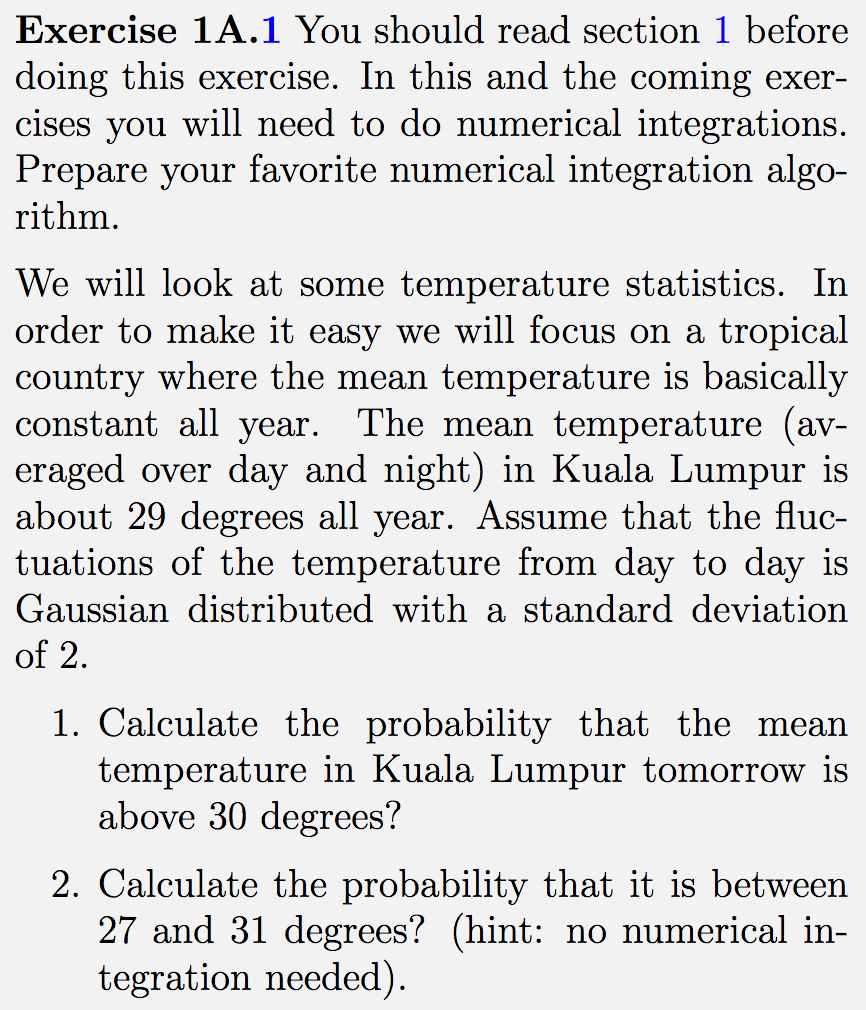
\includegraphics[scale=0.4]{media/screenshot_1a1.png}\\
\column{0.5\textwidth}
Tenk gjennom og diskuter hvordan du vil løse oppgavene. Du trenger ikke nødvendigvis løse de nå, men ha en klar ide om hvordan de kan løses...
Når du har det kan du gå til \hyperlink{stat8}{\pagebutton{Neste side}} {\bf Bruk maks 3 minutter til å tenke, finner du ikke ut av det, ta en kikk på hintet på neste side!}
\end{columns}
\end{frame}

\begin{frame}
\label{stat8}
\begin{columns}
\column{0.5\textwidth}
\lastpagebutton{stat7}
Hvis du er usikker på hvordan oppgavene løses, så kan du få et par hint i \href{https://www.uio.no/studier/emner/matnat/astro/AST2000/h20/undervisningsressurser/interaktive-forelesningsnotater/1a/videoer/video1a_11.mp4}{denne videoen}. Her er neste utfordring:
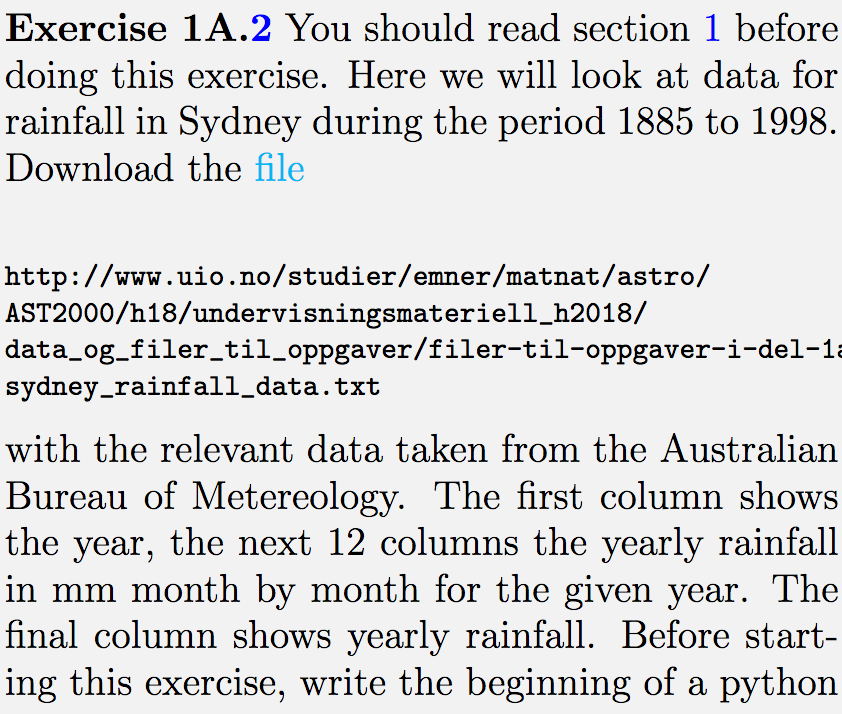
\includegraphics[scale=0.4]{media/screenshot_1a2_1.png}\\
\column{0.5\textwidth}
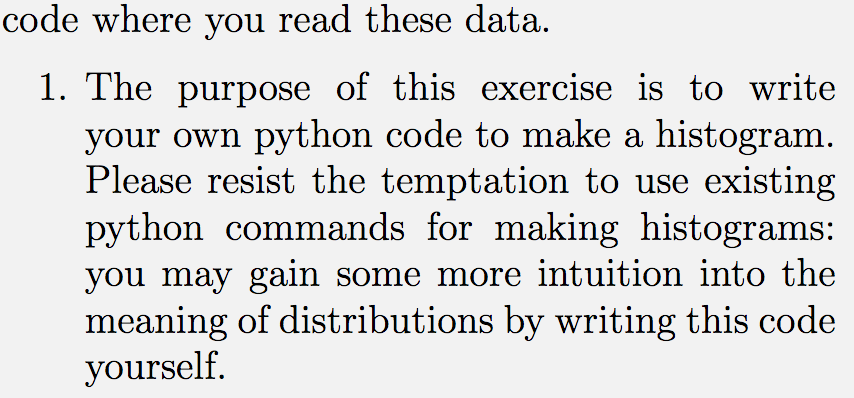
\includegraphics[scale=0.4]{media/screenshot_1a2_2.png}\\
Tenk igjen nøye gjennom hvordan du vil gå frem å løse dette. Det er viktig at du diskuterer denne med medstudenter. Her får du ikke noe svar, hvis du er veldig usikker, spør gruppelærer! {\bf Bergens tenketiden din til 3-4 minutter nå, fortsett senere når du skal gjøre oppgaven.}
\hyperlink{stat9}{\pagebutton{Neste side}}
\end{columns}
\end{frame}

\begin{frame}
\label{stat9}
\lastpagebutton{stat8}
Vi gir oss ikke med utfordringer her. Nå skal du prøve å oppdage en svært viktig statistisk regel gjennom å tenke deg frem til løsningen på denne utfordringen:
\begin{block}{\bf Hva iallverden har dette med astrofysikk å gjøre???}
Anta at $P(h$) er sannsynlighetsfordelingen for kroppshøyden $h$ til en person, anta også at $P(IQ)$ er sannsynlighetsfordelingen for IQ til en person. Anta at disse er Gaussike fordelinger (noe som stemmer rimelig godt). Ved å bruke disse fordelingene, hvordan kunne du regne ut sannsynligheten for at en tilfeldig valgt person har både høyde og IQ over gjennomsnittet? (anta at det ikke er noen sammenheng mellom å være høy og å være intelligent). Hvis du kjenner en spesiell statistisk regel for å gjøre dette, glem den regelen nå og bruk kun logisk resonnement for å finne svaret.\\
\end{block}
På de neste sidene skal du få se hva dette har med astrofysikk å gjøre, men først, tror du svaret er:\\
\hyperlink{feilprob}{\choicebutton{0\%}}\ \ \ \ \hyperlink{feilprob}{\choicebutton{20\%}}\ \ \ \ \hyperlink{rettprob}{\choicebutton{25\%}}\ \ \ \ \hyperlink{feilprob}{\choicebutton{50\%}}\\
\hyperlink{feilprob}{\choicebutton{60\%}}\ \ \ \ \hyperlink{feilprob}{\choicebutton{75\%}}\ \ \ \ \hyperlink{feilprob}{\choicebutton{90\%}}\ \ \ \ \hyperlink{feilprob}{\choicebutton{100\%}}\\
\end{frame}




{
\setbeamercolor{background canvas}{bg=black}
\begin{frame}
\label{feilprob}
\lastpagebutton{stat9}
\textcolor{white}{Det var nok ikke helt riktig! Trykk på tilbakeknappen og prøv igjen men ta med deg et hint på veien: anta at du har en gruppe på f.eks. 100 personer, hvor mange av disse har høyde over gjennomsnittet? Og hvor mange av disse har IQ over gjennomsnittet?}
\end{frame}
}

{
\setbeamercolor{background canvas}{bg=yellow}
\begin{frame}
\label{rettprob}
\clastpagebutton{stat9}
HELT RIKTIG!
Ta en kikk på \href{https://www.uio.no/studier/emner/matnat/astro/AST2000/h20/undervisningsressurser/interaktive-forelesningsnotater/1a/videoer/video1a_12.mp4}{denne videoen} nå for å lære en svært viktig regel for sannsynligheter og for å se hvordan du kan tenke for å komme frem til svaret på utfordringen. Ikke gå videre før du har forstått hva videoen prøver å forklare.
\hyperlink{centlimit}{\pagebutton{Neste side}}
\end{frame}
}


\begin{frame}
\label{centlimit}
\lastpagebutton{stat9}
{\small Du lurere kanskje på hvorfor vi antar Gaussisk fordeling for så mange forskjellige tilfeldige størrelser, fra hastigheter, til høyde og IQ? Svaret ligger blant annet i}
\begin{block}{\small Sentralgrenseteoremet (\small central limit theorem)}
{\small
Anta at du har $M$ sett av N uavhengige tilfeldige tall, dvs. du har M sett der hvert sett består at tilfeldige tall $x_1, x_2, ..., x_N$ som er trukket fra en nesten hvilken som helst foredelingsfunksjon, men alle tallene i alle M settene må være trukket fra den samme fordelingen. For hvert av de $M$ settene, ta midlet over de $N$ tallene i hvert sett og kall midlet $a_j$ ($j=[1,M]$). Gitt noen betingelser på fordelingsfunksjonen samt at $N$ er stor nok, så kan man vise matematisk at fordelingen til $a_j$ vil være tilnærmet Gaussisk. Under noen betingelser vil dette til og med være riktig hvis $x_1, x_2, ..., x_N$ er trukket fra forskjellige fordelinger. Du trenger ikke kjenne til detaljene og vi skal ikke diskutere disse betingelsene i AST2000.
}
\end{block}
{\small I veldig mange naturlige prosesser så tar man slike midler over mange tall implisitt, f.eks. hvis du måler temperaturen så tar du i realiteten midlet over temperaturene i løpet av et kort tidsrom. Dette gjør at mange tilfeldige tall fra naturlige og kompliserte prosesser har tilnærmet en enkel Gaussisk fordelingsfunksjon.}
\hyperlink{stat10}{\pagebutton{Neste side}}
\end{frame}


\begin{frame}
\label{stat10}
\lastpagebutton{centlimit}
Nå skal du øve deg på å bruke multiplikasjonsregelen for sannsynlighet. Vi begynner med gasser:
\begin{block}{\bf Maxwell-Boltzmannfordelingen for hastighetsvektor $\vec{v}$}
Hvordan kan du finne sannsynlighetsfordelingen for at en tilfeldig partikkel i en gass har hastighetsvektor $\vec{v}$? Du kan bruke de kjente fordelingene for $P(v_x)$, $P(v_y)$ og $P(v_z)$ samt multiplikasjonsregelen til å vise at
\[
P(\vec{v}) = \left(\frac{m}{2\pi kT}\right)^{3/2}e^{-\frac{1}{2}\frac{mv^2}{kT}}
\]
der $v=|\vec{v}|$.
\end{block}
Tenk i maks 2-3 minutter. Hvis du ikke ser hvordan det kan gjøres, ta en titt på \href{https://www.uio.no/studier/emner/matnat/astro/AST2000/h20/undervisningsressurser/interaktive-forelesningsnotater/1a/videoer/video1a_13.mp4}{denne videoen}.
\hyperlink{stat11}{\pagebutton{Neste side}}
\end{frame}

\begin{frame}
\label{stat11}
\begin{columns}
\column{0.5\textwidth}
\lastpagebutton{stat10}
La oss ta en titt på utdraget av resten av oppgave 1A.1:\\
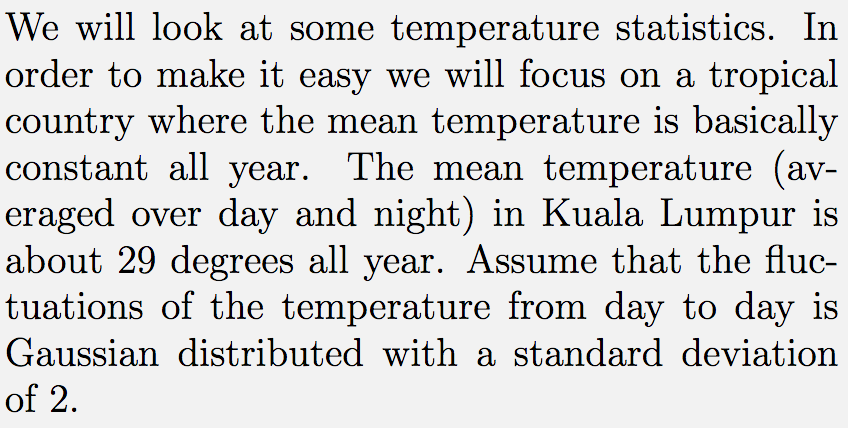
\includegraphics[scale=0.4]{media/screenshot_1a1_4.png}\\
\column{0.5\textwidth}
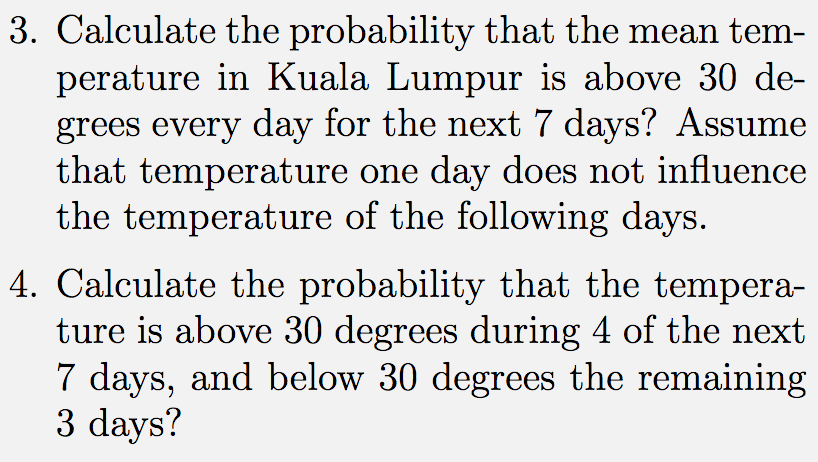
\includegraphics[scale=0.4]{media/screenshot_1a1_3.png}\\
Diskuter med medstudenter hvordan du kan løse disse oppgavene. For øyeblikket er det viktigste at du ser {\bf hvordan} du skal gå frem for å løse dette. {\bf Tenk i maks 1 minutt på hver deloppgave.}
\hyperlink{stat12}{\pagebutton{Neste side}}
\end{columns}
\end{frame}

\begin{frame}
\label{stat12}
\lastpagebutton{stat11}
Hvis du ikke så hvordan oppgaven på forrige side skulle løses, ta en titt på \href{https://www.uio.no/studier/emner/matnat/astro/AST2000/h20/undervisningsressurser/interaktive-forelesningsnotater/1a/videoer/video1a_14.mp4}{denne korte videoen} for litt hint.\\
Du har allerede (tidligere) brynet deg på den første deloppgaven av 1A.4. Ta en kikk nå på den andre:\\
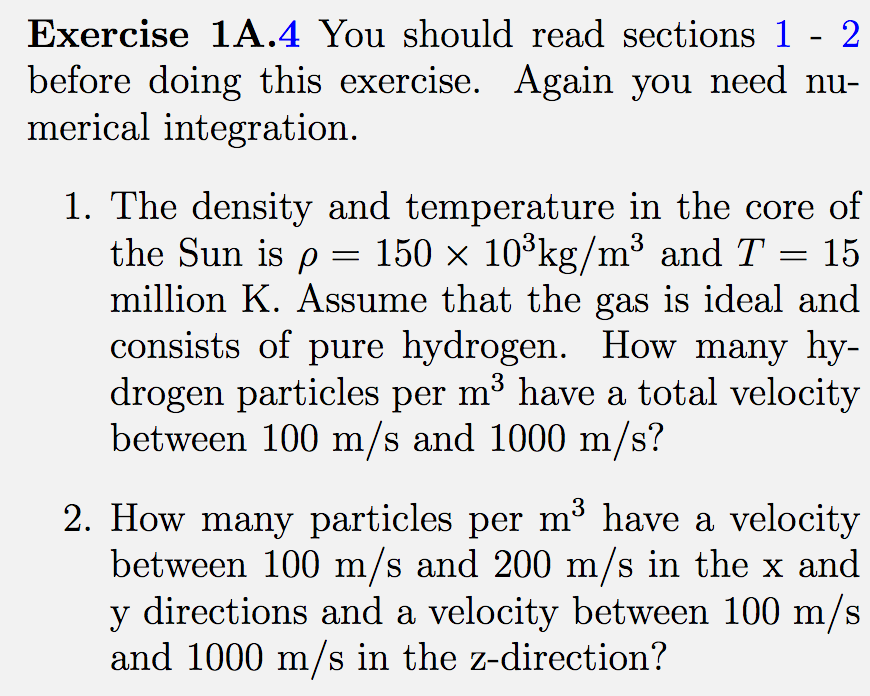
\includegraphics[scale=0.4]{media/screenshot_1a4_all.png}\\
Denne gangen får du ikke hjelp, spør gruppelærer hvis du er i tvil.\\
\hyperlink{stat13}{\pagebutton{Neste side}}
\end{frame}

\begin{frame}
\label{stat13}
\begin{columns}
\column{0.5\textwidth}
\lastpagebutton{stat12}
La oss nå gå tilbake til rakettmotoren vår i oppgave 1A6 (innleveringsoppgave).
 Utdrag fra oppgave 1A6:\\
 \vspace{0.5cm}
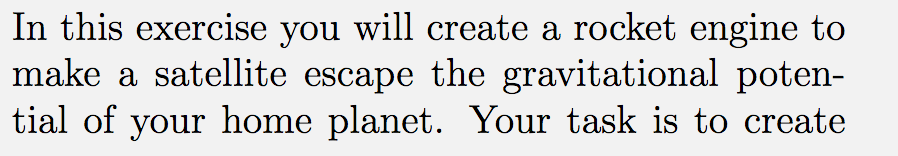
\includegraphics[scale=0.35]{media/1a6_1.png}
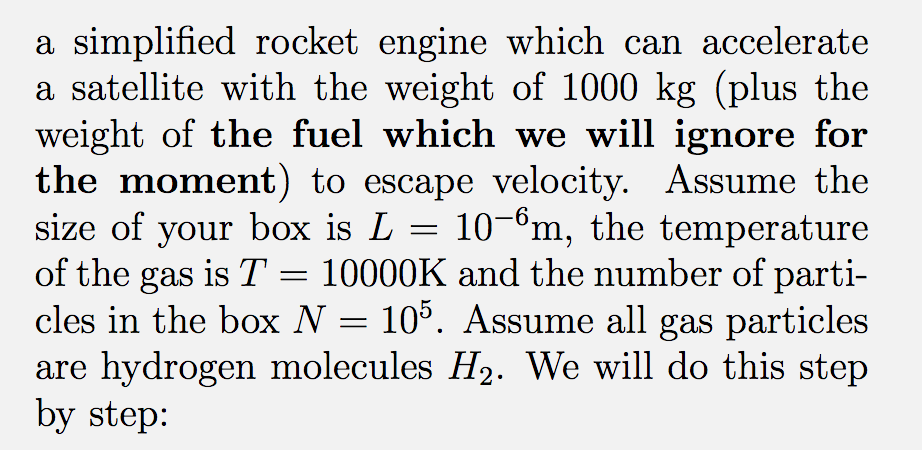
\includegraphics[scale=0.35]{media/1a6_2.png}\\
\column{0.5\textwidth}
Vi skal nå se på andre deloppgave:\\
\vspace{0.5cm}
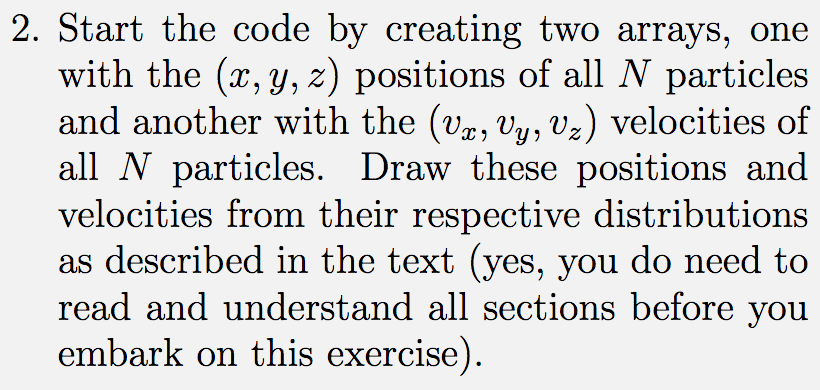
\includegraphics[scale=0.35]{media/1a6_3.png}\\
Her kan du få bruk for \href{https://docs.python.org/2/library/random.html}{random-klassen (link)} i python. Spesielt bør du lese om \href{https://pynative.com/python-random-seed/}{\tt random.seed}, \href{https://kite.com/python/docs/random.gauss}{\tt random.gauss} og \href{https://kite.com/python/docs/random.uniform}{\tt random.uniform}.
Er du enda usikker på hvordan du skal gjøre dette, så kan du få noen hint i \href{https://www.uio.no/studier/emner/matnat/astro/AST2000/h20/undervisningsressurser/interaktive-forelesningsnotater/1a/videoer/video1a_15.mp4}{denne videoen}
\hyperlink{pause}{\pagebutton{Neste side}}
\end{columns}
\end{frame}

{
\setbeamercolor{background canvas}{bg=cyan}
\begin{frame}
\label{pause}
\hyperlink{stat13}{\pagebutton{\small Forrige side}}
{\huge
\centerline{Kaffe?}
\centerline{
\includegraphics[scale=4]{media/drink-coffee.png}}\\
\small Tiden har kommet for en god strekk på bena! Og helle på med en mørk væske som har høye partikkelhastigheter. Ta deg en ekstra god pause nå, fordi du etter pausen for alvor skal begynne å se på konstruksjon av rakettmotoren din.
}\\
\vspace*{0.5cm}
\hyperlink{ideelgass1}{\pagebutton{Ok, jeg begynner å bli klar for romreise...}}
\end{frame}
}

\begin{frame}
\label{ideelgass1}
\lastpagebutton{stat13}
Nå som vi vet hvordan lage gasspartiklene i rakettmotoren vår, så gjenstår noen få men svært viktige temaer før vi kan sette igang å bevege partiklene slik at det faktisk blir en virtuell gass. Vi kjenner nå hastighetene til partiklene våre, og mens partiklene ikke støter på noen vegg eller på andre partikler så forblir denne hastigheten uforandret. Dermed er det i første omgang ganske greit å bevege partiklene i løpet av et lite tidssteg. Men etterhvert kommer de til å kollidere, og det er da vi trenger \textcolor{red}{antakelsen om ideel gass} (litt forenklet):
\begin{itemize}
\item det er ingen interaksjon mellom partiklene
\item kollisjonen med veggene er {\it elastisk}
\end{itemize}
De aller fleste gasser der temperaturen ikke er veldig høy eller veldig lav er gode tilnærmelser til ideele gasser.
Men hva innebærer \textcolor{red}{elastiske kollisjoner}? Kan du huske det fra mekanikken? Tenk nøye gjennom det før du går videre!
\hyperlink{ideelgass2}{\pagebutton{Neste side}}
\end{frame}

\begin{frame}
\label{ideelgass2}
\lastpagebutton{ideelgass1}
I en \textcolor{red}{elastiske kollisjon}, så er ... \hyperlink{elkoll}{\pagebutton{Trykk her}}
\pause
\addtocounter{pageno}{-1}
\begin{itemize}[<+->]
\item[] ... den kinetiske energien til partiklene den samme før og etter kollisjonen ... \hypertarget<.>{elkoll}{}
\end{itemize}
Det betyr at absoluttverdien av bevegelsesmengden ... \hyperlink{elkoll2}{\pagebutton{Trykk her}}
\pause
\begin{itemize}[<+->]
\item[] ... også er den samme før og etter kollisjonen (ser du det???) \hypertarget<.>{elkoll2}{}
\end{itemize}
\href{https://www.uio.no/studier/emner/matnat/astro/AST2000/h20/undervisningsressurser/interaktive-forelesningsnotater/1a/animasjoner/particle_simulation_general.mov?vrtx=view-as-webpage}{Se på disse kollisjonene her mellom gasspartikler og vegg...}\\

Hva skjer med bevegelsesmengdene $p_x$ og $p_y$ i x- og y-retning her hvis kollisjonene er ellastiske?\\

Når du vet svaret, gå til \hyperlink{ideelgass3}{\pagebutton{Neste side}}
\end{frame}

\begin{frame}
\label{ideelgass3}
\dlastpagebutton{ideelgass2}
{\small
{\bf La oss se på en partikkel som kolliderer med veggen på høyre side slik at hastigheten i x-retning bytter retning.} Er du enig i at det i y-retning (opp-ned-retning) ikke virker noen krefter i denne kollisjonen?
\hyperlink{elkoll3}{\pagebutton{Trykk her når du er enig}}
\pause
\addtocounter{pageno}{-2}
\begin{itemize}[<+->]
\item[] \hypertarget<.>{elkoll3}{}
\end{itemize}
\vspace*{-0.5cm}
Er du dermed enig i at bevegelsesmengde i y-retning, $p_y$, er uendret? 
\hyperlink{elkoll4}{\pagebutton{Trykk her når du er enig}}
\pause
\begin{itemize}[<+->]
\item[]  \hypertarget<.>{elkoll4}{}
\end{itemize}
\vspace*{-0.5cm}
Er du også enig i at absoluttverdien av bevegelsesmengden i x-retning må være uendret pga. elastisk kollisjon?
\hyperlink{elkoll5}{\pagebutton{Trykk her når du er enig}}
\pause
\begin{itemize}[<+->]
\item[] \hypertarget<.>{elkoll5}{}
\end{itemize}
\vspace*{-0.5cm}
 Er du også enig i at fortegnet til bevegelsesmengde i x-retning er endret?
\hyperlink{elkoll6}{\pagebutton{Trykk her når du er enig, ikke før!}}
\pause
\begin{itemize}[<+->]
\item[]  \hypertarget<.>{elkoll6}{}
\end{itemize}
\vspace*{-0.5cm}
Er du da også enig i at ...
\begin{eqnarray}
p_x\mathrm{(etter\  kollisjon)} &= \textcolor{red}{\textbf{-}} p_x\mathrm{(før\  kollisjon)}\\
p_y\mathrm{(etter\  kollisjon)} &= p_y\mathrm{(før\  kollisjon)}
\end{eqnarray}
Hvis du er uenig i noe av det over, spør foreleser/gruppelærer \hyperlink{ideelgass3b}{\pagebutton{Neste side}}
}
\end{frame}


\begin{frame}
\label{ideelgass3b}
\addtocounter{pageno}{1}
\dlastpagebutton{ideelgass3}
Her ser vi situasjonen illustrert:\\
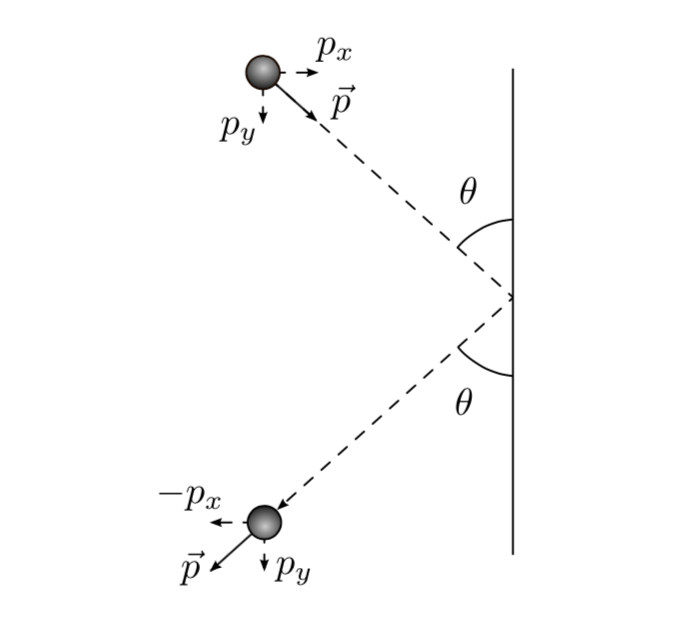
\includegraphics[scale=0.6]{media/elcol.png}\\
\hyperlink{trykk1}{\pagebutton{Neste side}}
\end{frame}

\begin{frame}
\label{trykk1}
\lastpagebutton{ideelgass3b}
Kan du definere gasstrykk?
Kikk på \href{https://www.uio.no/studier/emner/matnat/astro/AST2000/h20/undervisningsressurser/interaktive-forelesningsnotater/animasjoner/particle_simulation_pressure_forces.mov?vrtx=view-as-webpage}{denne videoen} for å se om den kan hjelpe deg med å finne en definisjon.
Tenk deg om før du \hyperlink{trykkbutton1}{\pagebutton{trykker på denne knappen}}
\pause
\addtocounter{pageno}{-1}
\begin{itemize}[<+->]
\item[]  Er du enig i at partiklene utøver en kraft på veggen hver gang de treffer?\hypertarget<.>{trykkbutton1}{}
\end{itemize}
Kan det hjelpe deg litt med definisjonen?
Tenk deg om igjen og \hyperlink{trykkbutton2}{\pagebutton{trykk på denne knappen}}
\pause
\begin{itemize}[<+->]
\item[]  Definisjon: \hypertarget<.>{trykkbutton2}{}
\end{itemize}
\begin{alertblock}{\bf Gasstrykk er ...}
Den totale kraften fra partiklene per areal, altså:
\[
P = \frac{F}{A}
\]
der $P$ er gasstrykk som måles i N/m$^2$ også kalt Pa (Pascal).\hyperlink{trykk2}{\pagebutton{Neste side}}
\end{alertblock}

\end{frame}

\begin{frame}
\label{trykk2}
\dlastpagebutton{trykk1}
\textcolor{red}{\underline{La oss se om vi kan finne et uttrykk for gasstrykket:}}\\
Kraft kan skrives som 
\[
F = \frac{\Delta p}{\Delta t}
\]
altså endring i bevegelsesmengde per tid. Hvilken endring $\Delta p$ i bevegelsesmengde får en gasspartikkel med masse $m$ og x-hastighet $v_x$ på veggen ved kollisjon (anta ideel gass og dermed elastisk kollisjon)? {\bf (Bruk maks 2 min. til å tenke!)} \\
\hyperlink{feilp}{\choicebutton{$|\Delta p| = mv_x$}}\ \ \ \ \hyperlink{feilp}{\choicebutton{$|\Delta p| = mv_x^2$}}\ \ \ \ \hyperlink{riktigp}{\choicebutton{$|\Delta p| = 2mv_x$}}\ \ \ \ \hyperlink{feilp}{\choicebutton{$|\Delta p| = \frac{1}{2}mv_x^2$}}\ \ \ \ \hyperlink{feilp}{\choicebutton{$|\Delta p| = 4mv_x$}}\\
\end{frame}


{
\setbeamercolor{background canvas}{bg=black}
\begin{frame}
\label{feilp}
\lastpagebutton{trykk2}
\textcolor{white}{Det var nok ikke helt riktig! Trykk på tilbakeknappen og prøv igjen men ta med deg et hint på veien: Endring i bevegelsesmengde er lik bevegelsesmengden etter minus bevegelsesmengde før, enig? Altså:
\[
\Delta p = p\mathrm{(etter)} - p\mathrm{(før)}
\]
Men hva er bevegelsesmengde før og etter kollisjon? (husk fortegn her!)}
\end{frame}
}

{
\setbeamercolor{background canvas}{bg=yellow}
\begin{frame}
\label{riktigp}
\clastpagebutton{trykk2}
HELT RIKTIG!
Du har sikkert tenkt slik:
Endring i bevegelsesmengde er lik bevegelsesmengden etter minus bevegelsesmengde før, enig? Altså:
\[
\Delta p = p\mathrm{(etter)} - p\mathrm{(før)} = -mv_x - mv_x = -2mv_x=-2p_x
\]
Kraften som en partikkel utøver på veggen ved kollisjoner altså
\[
f = \frac{\Delta p}{\Delta t} = \frac{2p_x}{\Delta t}
\]
Men hva skal vi bruke som tiden her??? For å komme videre slik at vi kan finne et uttrykk for gasstrykket så trenger vi denne.
For å finne ut av dette og dermed kunne utlede gasstrykket, så skal vi se på et bittelite volum $dV$ av gass rett ved en vegg. Vi antar at det lille volumet vårt har form som en sylinder eller som en rektangulær boks med lengde $\Delta x$ og endesideflater med areal $A$. \\
På neste side skal vi se nærmere på boksen...
\hyperlink{trykk3}{\pagebutton{Neste side}}
\end{frame}
}

\begin{frame}
\label{trykk3}
\lastpagebutton{trykk2}
Her er den:\\
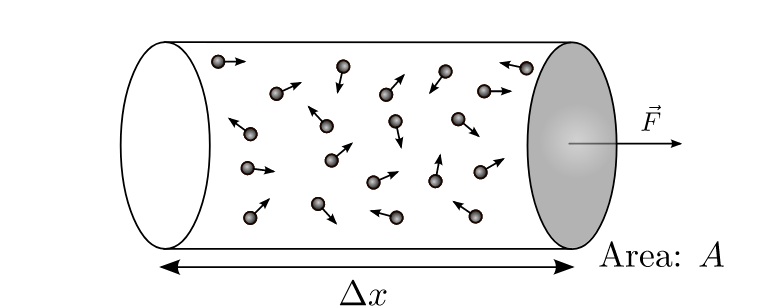
\includegraphics[scale=0.5]{media/cylinder.png}\\
Vi skal nå beregne den totale tiden det tar for alle partiklene i denne boksen å ha truffet veggen som ligger på høyre side av boksen.
Først skal vi kun se på partiklene som har en gitt absoluttverdi $v_x$ av hastigheten. Du kan se disse partiklene i \href{https://www.uio.no/studier/emner/matnat/astro/AST2000/h20/undervisningsressurser/interaktive-forelesningsnotater/animasjoner/particle_simulation_pressure_integral.mov?vrtx=view-as-webpage}{denne videoen}.
De røde partiklene er de med hastighet $v_x$ på vei mot veggen på høyre side, de blå partiklene har hastighet $-v_x$ og er på vei vekk fra veggen (dvs. de har allerede kollidert med veggen tidligere.
\hyperlink{trykk4}{\pagebutton{Neste side}}
\end{frame}

\begin{frame}
\label{trykk4}
\lastpagebutton{trykk3}
Hvor lang tid tar det før alle de røde partiklene har truffet veggen? (husk $\Delta x$ er lengden av boksen, $v_x$ er absoluttverdi av hastighetskomponent i x-retning som er lik for alle partikler og $A$ er arealet av endesideflatene)\\
Se gjerne \href{https://www.uio.no/studier/emner/matnat/astro/AST2000/h20/undervisningsressurser/interaktive-forelesningsnotater/animasjoner/particle_simulation_pressure_integral.mov?vrtx=view-as-webpage}{videoen igjen}. {\bf (Bruk maks 2 min. til å tenke!)}\\
\hyperlink{feilt}{\choicebutton{$\Delta t = v_x \Delta t$}}\ \ \ \ \hyperlink{feilt}{\choicebutton{$\Delta t = \frac{v_x}{A}$}}\ \ \ \ \hyperlink{feilt}{\choicebutton{$\Delta t = \frac{v_x}{\Delta x}$}}\ \ \ \ \hyperlink{riktigt}{\choicebutton{$\Delta t = \frac{\Delta x}{v_x}$}}\ \ \ \ \hyperlink{feilt}{\choicebutton{$\Delta t = 2v_x\Delta x$}}
\end{frame}


{
\setbeamercolor{background canvas}{bg=black}
\begin{frame}
\label{feilt}
\lastpagebutton{trykk4}
\textcolor{white}{Det var nok ikke helt riktig! Trykk på tilbakeknappen og prøv igjen men ta med deg et hint på veien: Er du enig i at den røde partikkelen helt til venstre er den siste som treffer veggen? Den trenger å gå en avstand $\Delta x$ i x-retning med en hastighet $v_x$. }
\end{frame}
}

{
\setbeamercolor{background canvas}{bg=yellow}
\begin{frame}
\label{riktigt}
\clastpagebutton{trykk4}
HELT RIKTIG!\\
Når den røde partikkelen helt til venstre har truffet veggen, så har alle røde partikler truffet veggen. Partikkelen trenger å gå en avstand $\Delta x$ i x-retning med en hastighet $v_x$, dermed tar det den tid $\Delta x/v_x$. Men vi må også se hvor lang tid de blå partiklene har brukt for å treffe veggen! Disse er på vei bort fra veggen og har dermed truffet veggen tidligere, men hvor lang tid tok det for alle de blå partiklene å treffe veggen? Kan du bruke samme type resonnement?
Hvis du ikke ser det, \hyperlink{trykkbutton3}{\pagebutton{trykk her for et tips}}
\pause
\begin{itemize}[<+->]
\item[] Den blå ballen helt til venstre er vel den første som traff veggen? \hypertarget<.>{trykkbutton3}{}
\end{itemize}
Hvor lang tid er det siden i det videoen starter?
Ikke gå til neste side før du har svaret!
\hyperlink{trykk5}{\pagebutton{Neste side}}
\end{frame}
}


\begin{frame}
\label{trykk5}
\lastpagebutton{trykk4}
Den blå ballen til venstre har beveget seg en strekning i negativ x-retning på $\Delta x$ siden den traff veggen med hastighet $v_x$, den traff dermed veggen en tid $\Delta x/v_x$ før videoen starter. Alle andre blå baller traff senere, altså kortere tid siden, fordi disse enda er nærmere veggen.\\
 Konklusjonen vår er at alle ballene i boksen traff veggen i løpet av totalt tiden $2\Delta x/v_x$. Og de 'la igjen' en bevegelsemengde $N\times2p_x$ der $N$ er antall partikler, Total kraft på veggen er dermed
\[
F = \frac{\Delta p}{\Delta t} = N\times\frac{2p_x}{2\Delta x/v_x} = \frac{Nv_xp_x}{\Delta x}
\]
I \href{https://www.uio.no/studier/emner/matnat/astro/AST2000/h20/undervisningsressurser/interaktive-forelesningsnotater/1a/videoer/video1a_16.mp4}{denne videoen} tar vi dette uttrykket videre og utleder trykkintegralet:
\[
P = \frac{1}{3}\int_0^\infty vp\;n(p)dp,
\]
der $v$ er hastigheten som tilsvarer bevegelsesmengden $p$ (som er $p=mv$ hvis ikke-relativistisk) og $n(p)$ er fordelingsfunksjonen som sier hvor mange partikler per volum som har bevegelsesmengde i intervallet $[p,p+dp]$, for ideel gass tilsvarer dette Maxwell-Boltzmann.
\hyperlink{pnkt}{\pagebutton{Neste side}}
\end{frame}



\begin{frame}
\label{pnkt}
\lastpagebutton{trykk5}
I deloppgave 2 i 1A.4 skal du analytisk integrere opp trykklintegralet for ideel gass med $p=mv$ og $n(p)$ som Maxwell-Boltzmann. Resultatet du får er svært viktig i termodynamikk:
\begin{alertblock}{\bf Tilstandslikningen for ideel gass}
Tilstandslikningen (equation of state) til en gass er en sammenheng mellom trykk, temperatur og tetthet. For en ideel gass er denne:
\[
P = nkT
\]
der $n$ er antalltettheten av gassen, altså totalt antall gasspartikler per volum, $k$ er \href{https://no.wikipedia.org/wiki/Boltzmanns_konstant}{Boltzmannkonstanten} og $T$ er temperaturen til gassen. 
\end{alertblock}
Denne sammenhengen kommer vi til å bruke igjen og igjen, så lær den med en gang.
\hyperlink{rakettmotor1}{\pagebutton{Neste side}}
\end{frame}

\begin{frame}
\label{rakettmotor1}
\lastpagebutton{pnkt}
Så tilbake til rakettmotoren vår. Nå har vi alt vi trenger. Du har allerede laget partiklene med posisjoner og hastigheter, da må du
\begin{enumerate}
\item bevege hver partikkel fremover i hvert tidssteg
\item sjekke om du treffer en vegg
\item nå har du sett hva du kan gjøre når du får en ellastisk kollisjon
\item sjekk om du treffer hullet i boksen, da går partikkelen ut, men du må få en ny partikkel inn i boksen igjen for å passe på å holde tetthet og temperatur konstant.
\item beregne rakettens akselrasjon for hver partikkel som går ut av hullet
\end{enumerate}
Siden vi holder temperatur og tetthet i boksen konstant, kan du beregne rakettens akselrasjon for et veldig kort tidsrom, og så bruke denne akseprasjonen videre i beregningene. Du trenger dermed kun å simulere boksen for et kort tidsrom for å finne ut hvor mye akselrasjon raketten får per tid. Merk at boksen også er {\bf alt} for liten til å drive en hel rakett, du trenger et {\bf meget stort} antall slike bokser, du trenger altså å gange opp akselrasjonen fra en boks med antall bokser.
\hyperlink{rakettmotor1b0}{\pagebutton{Neste side}}
\end{frame}

\begin{frame}
\label{rakettmotor1b0}
\lastpagebutton{rakettmotor1}
I oppgaven skal du få raketten opp i {\bf unnslippingshastighet (escape velocity)}. Men hva er unnslippingshastighet? Det er hastigheten der rakettens kinetiske energi er større en jordas potensielle slik at den ikke lenger faller tilbake til jorda. Ser du hvordan du kan beregne den?\hyperlink{escvel1}{\pagebutton{Trykk her når du har tenkt!}}
\pause
\begin{itemize}[<+->]
\item[]  \hypertarget<.>{escvel1}{}
\end{itemize}
\vspace*{-0.5cm}
Svaret du skal få er
\[
v_\mathrm{esc}=\sqrt{\frac{2GM}{R}}
\]
der $R$ er avstanden fra jordas sentrum der hastigheten når $v_\mathrm{esc}$ og $M$ er jordas masse. Fikk du det? Hvis ikke, spør foreleser/gruppelærer!
\hyperlink{rakettmotor1b}{\pagebutton{Neste side}}
\end{frame}


\begin{frame}
\label{rakettmotor1b}
\lastpagebutton{rakettmotor1}
{\bf\large Men hva gjør du hvis koden ikke funker som den skal?\\
Hva hvis den gir rare resultater for fremdrift, trykk, energi etc.? Hva gjør du da?}
\hyperlink{fdebug}{\choicebutton{\small Kikker gjennom koden noen ganger for å se om jeg ser noe feil}}\ \ \ \ \hyperlink{rdebug}{\choicebutton{\small Bruker litt grunnleggende fysikk for å finne hvor feilen ligger}}\
\end{frame}

{
\setbeamercolor{background canvas}{bg=black}
\begin{frame}
\label{fdebug}
\lastpagebutton{rakettmotor1b}
\textcolor{white}{Lykke til! Det kan du trenge, for dette kan ta laaaaaaaaaaaaaang tid!\\}
\hyperlink{rdebug}{\pagebutton{\small Trykk her for noen tips til hvodan dette kan ta mye kortere tid}}
\end{frame}
}

{
\setbeamercolor{background canvas}{bg=yellow}
\begin{frame}
\label{rdebug}
\clastpagebutton{rakettmotor1b}
Det er veldig lurt å lære noen tips til hvordan du kan bruke litt fysikk til å debugge en kode. Her er noen tips hvis gassboksen og/eller rakettmotoren ikke gir de resultater som du forventer. Vi begynner med gassboks {\bf uten hull}.
{\small
\begin{enumerate}
\item lag histogram av hastigheten til partiklene og plott Maxwell-Boltzmann over, stemmer det sånn omtrent?
\item Hvordan vil hastighetskomponentene til partiklene se ut som funksjon av tiden? Det vet du med litt fysikk. Velg deg ut en av partiklene i gassen og lag 3 lister med  $v_x$, $v_y$ og $v_z$-komponenten i hvert tidssteg gjennom hele simuleringen. Plott disse. Er de slik som de skal være?
\item Hvis ikke, hvor begynner hastighetskomponenten(e) å oppføre seg rart? Er det f.eks. etter første kollisjon med vegg? Hva er det ellers som kan endre hastighetskomponentene?
\item Hvis alt stemmer med hastighetskomponentene, lag 3 lister med x, y og z-posisjonene for en valgt partikkel for alle tidssteg. Plot posisjonene som funksjon av tiden. Er posisjonene slik du forventer? Er posisjonsendringer ved veggtreff synkronisert med hastighetsendringer? Går posisjonene utenfor boksen?
\end{enumerate}
}
\hyperlink{rakettmotor2}{\pagebutton{Neste side}}
\end{frame}
}

\begin{frame}
\label{rakettmotor2}
\lastpagebutton{rdebug}
Og det bringer oss tilbake til spørsmålet vi hadde helt i starten!
\begin{enumerate}
\item Hvor mye bevegelsesmengde slipper ut av hullet for hver partikkel som slipper ut?
\item Hvordan kan den bevegelsesmengden som slipper ut hjelpe deg til å finne rakettens akselrasjon? (finnes det en sammenheng mellom kraft og endring i bevegelsesmengde?)
\item Pass på retningen til bevegelsesmengden for hver partikkel som kommer ut og retningen til raketten.
\item Når du har akselrasjonen, hvordan går du så frem for å finne rakettens posisjon som funksjon av tid etter oppskyting?
\end{enumerate}
Svarene får du ikke her! Hvis du ikke finner ut av det, få hjelp på gruppene!
\hyperlink{rakettmotor2b}{\pagebutton{Neste side}}
\end{frame}

\begin{frame}
\label{rakettmotor2b}
\clastpagebutton{rakettmotor2}
Hvis nå motoren uten hull gir fornuftig trykk, midlere partikkelenergi etc., da kan vi sjekke motoren med hull: hvis du får for lite/for mye fremdrift eller ingen i det hele tatt, så kan du f.eks.
{\small
\begin{enumerate}
\item lage histogram av x,y og z-komponentene for alle partikkelposisjonene og hastighetene i første og siste tidssteg. Er hastightene enda omtrent Maxwell-boltzmann fordelt? Kan være litt avvik her avhengig av hvordan du regenererer partikler, men hvis du har veldig mange partikler med veldig liten/stor hastighet, så er noe galt med måten du gir hastighet til de nye partiklene som erstatter de som forsvinner ut. Er posisjonene enda uniformt fordelt? Hvis ikke er noe galt med måten du gir posisjon/hastighet til nygenererte partikler.
\item slipper noen/nok/for mange partikler ut av hullet? Kan det være en feil i hvordan du sjekker om partiklene slipper ut av hullet? Etter å ha generert partikkelposisjoner og hastigheter helt i starten, forandre posisjon og hastighet til en valgt partikkel slik at den står rett ved utgangen av hullet med hastighet ut av hullet. Sjekk så om partikkelen med dette indeksnummeret faktisk slipper ut av boksen. Hvis ikke: lag lister med posisjoner/hastigheter i alle tidssteg og sjekk hva som skjer mens den egentlig skulle slippe ut av hullet (som på forrige side). Er betingelsen din for at den har gått ut av hullet faktisk blitt oppfylt?\hyperlink{sammendrag}{\pagebutton{\small Neste side}}
\end{enumerate}
}
\end{frame}


\begin{frame}
\label{sammendrag}
\lastpagebutton{rakettmotor2b}
{\scriptsize
Gratulerer, du er ferdig med Del 1A av AST2000. Dette bør du nå kunne svare på før du går videre:
\begin{enumerate}
\item Hva er, og hvordan bruker man, en statistisk fordelingsfunksjon? (eller sannsynlighetstetthet)
\item Hva er, og hvordan beregner man, gjennomsnitt, standardavvik, varianse, FWHM?
\item Hva er en Gaussisk sannsynlighetsfordeling og hva er sannsynligheten for å trekke en verdi innenfor $1\sigma$, $2\sigma$ og $3\sigma$ fra gjennomsnittet?
\item Hva er en ideel gass?
\item Hvordan kan du finne fordelingen av partikkelhastigheter i en ideel gass?
\item Hva er trykk, hvordan kan du beregne trykk analytisk og numerisk og hva er tilstandslikning for ideel gass?
\item Hva gjør at en rakett akselererer?
\item Hvordan går du frem for å beregne egenskapene en gass trenger i en rakettmotor for å få en gitt akselrasjon?
\end{enumerate}
    {\bf Det anbefales nå at du sjekke \href{https://www.uio.no/studier/emner/matnat/astro/AST2000/h21/undervisningsmateriell/kortsvarsoppgaver/del1a.pdf}{kortsvarsoppgavene} til del 1A for å kontrollere at du har forstått stoffet. Kan du svare på disse, blir det lettere å bruke kunnskapen din i oppgavene/prosjektet. Noen av disse kommer på eksamen.}
    }
\end{frame}

\end{document}

